\documentclass[12pt, twoside]{book}
%\documentclass[12pt, oneside]{book}  % jednostranna tlac
\usepackage[a4paper,top=2.5cm,bottom=2.5cm,left=3.5cm,right=2cm]{geometry}
\usepackage[utf8]{inputenc}
\usepackage[T1]{fontenc}
\usepackage{graphicx}
\usepackage{url}
\usepackage[hidelinks,breaklinks]{hyperref}
\usepackage{float}
\usepackage{hyperref} % https://texblog.org/2012/03/21/cross-referencing-list-items/

% Adapted from: https://mysnippets443.wordpress.com/2015/11/28/latex-insert-javascript-code-with-lstlisting-package/
\usepackage{listings} % https://www.overleaf.com/learn/latex/Code_listing
\usepackage{color} %use color
\definecolor{mygreen}{rgb}{0,0.6,0}
\definecolor{mygray}{rgb}{0.5,0.5,0.5}
\definecolor{mymauve}{rgb}{0.58,0,0.82}
%Customize a bit the look
\lstset{ %
backgroundcolor=\color{white}, % choose the background color; you must add \usepackage{color} or \usepackage{xcolor}
basicstyle=\footnotesize, % the size of the fonts that are used for the code
breakatwhitespace=false, % sets if automatic breaks should only happen at whitespace
breaklines=true, % sets automatic line breaking
captionpos=b, % sets the caption-position to bottom
commentstyle=\color{mygreen}, % comment style
deletekeywords={...}, % if you want to delete keywords from the given language
escapeinside={\%*}{*)}, % if you want to add LaTeX within your code
extendedchars=true, % lets you use non-ASCII characters; for 8-bits encodings only, does not work with UTF-8
frame=single, % adds a frame around the code
keepspaces=true, % keeps spaces in text, useful for keeping indentation of code (possibly needs columns=flexible)
keywordstyle=\color{blue}, % keyword style
% language=Octave, % the language of the code
morekeywords={*,...}, % if you want to add more keywords to the set
numbers=none, % where to put the line-numbers; possible values are (none, left, right)
numbersep=5pt, % how far the line-numbers are from the code
numberstyle=\tiny\color{mygray}, % the style that is used for the line-numbers
rulecolor=\color{black}, % if not set, the frame-color may be changed on line-breaks within not-black text (e.g. comments (green here))
showspaces=false, % show spaces everywhere adding particular underscores; it overrides 'showstringspaces'
showstringspaces=false, % underline spaces within strings only
showtabs=false, % show tabs within strings adding particular underscores
stepnumber=0, % the step between two line-numbers. If it's 1, each line will be numbered
stringstyle=\color{mymauve}, % string literal style
tabsize=2, % sets default tabsize to 2 spaces
title=\lstname % show the filename of files included with \lstinputlisting; also try caption instead of title
}
%END of listing package%
\definecolor{darkgray}{rgb}{.4,.4,.4}
\definecolor{purple}{rgb}{0.65, 0.12, 0.82}
%define Javascript language
\lstdefinelanguage{JavaScript}{
keywords={typeof, new, true, false, catch, function, return, null, catch, switch, var, if, in, while, do, else, case, break},
keywordstyle=\color{blue}\bfseries,
ndkeywords={class, export, boolean, throw, implements, import, this},
ndkeywordstyle=\color{darkgray}\bfseries,
identifierstyle=\color{black},
sensitive=false,
comment=[l]{//},
morecomment=[s]{/*}{*/},
commentstyle=\color{purple}\ttfamily,
stringstyle=\color{red}\ttfamily,
morestring=[b]',
morestring=[b]"
}
\lstset{
language=JavaScript,
extendedchars=true,
basicstyle=\footnotesize\ttfamily,
showstringspaces=false,
showspaces=false,
numbers=left,
numberstyle=\footnotesize,
numbersep=9pt,
tabsize=2,
breaklines=true,
showtabs=false,
captionpos=b
}

%\usepackage[slovak]{babel} % vypnite pre prace v anglictine
\linespread{1.25} % hodnota 1.25 by mala zodpovedat 1.5 riadkovaniu

% CUSTOM THINGS
\newtheorem{theorem}{Definition}[section]
\newtheorem{corollary}{Corollary}[theorem]
\newtheorem{lemma}[theorem]{Lemma}
\usepackage{amsmath}

% -------------------
% --- Definicia zakladnych pojmov
% --- Vyplnte podla vasho zadania
% -------------------
\def\mfrok{2021}
\def\mfnazov{Trusted Types integration into open source frameworks and libraries}
\def\mftyp{Masters Thesis}
\def\mfautor{Emanuel Tesař, Bc.}
\def\mfskolitel{RNDr. Peter Borovanský, PhD.}

%ak mate konzultanta, odkomentujte aj jeho meno na titulnom liste
\def\mfkonzultant{Krzysztof Kotowicz}

\def\mfmiesto{Bratislava, \mfrok}

% bioinformatici odkomentujú riadok s dvoma odbormi a iný program
\def\mfodbor{Computer Science}
%\def\mfodbor{Computer Science and Biology}
\def\program{Computer Science}
%\def\program{ Bioinformatics }

% Ak je školiteľ z FMFI, uvádzate katedru školiteľa, zrejme by mala byť aj na zadaní z AIS2
% Ak máte externého školiteľa, uvádzajte Katedru informatiky
\def\mfpracovisko{ FMFI.KAI - Department of Applied Informatics }

\begin{document}
\frontmatter


% -------------------
% --- Obalka ------
% -------------------
\thispagestyle{empty}

\begin{center}
  \sc\large
  Comenius University in Bratislava\\
  Faculty of Mathematics, Physics and Informatics

  \vfill

  {\LARGE\mfnazov}\\
  \mftyp
\end{center}

\vfill

{\sc\large
  \noindent \mfrok\\
  \mfautor
}

\cleardoublepage
% --- koniec obalky ----

% -------------------
% --- Titulný list
% -------------------

\thispagestyle{empty}
\noindent

\begin{center}
  \sc
  \large
  Comenius University in Bratislava\\
  Faculty of Mathematics, Physics and Informatics

  \vfill

  {\LARGE\mfnazov}\\
  \mftyp
\end{center}

\vfill

\noindent
\begin{tabular}{ll}
  Study Programme: & \program      \\
  Field of Study:  & \mfodbor      \\
  Department:      & \mfpracovisko \\
  Supervisor:      & \mfskolitel   \\
  Consultant:      & \mfkonzultant \\
\end{tabular}

\vfill


\noindent \mfmiesto\\
\mfautor

\cleardoublepage
% --- Koniec titulnej strany


% -------------------
% --- Zadanie z AIS
% -------------------
% v tlačenej verzii s podpismi zainteresovaných osôb.
% v elektronickej verzii sa zverejňuje zadanie bez podpisov
% v pracach v naglictine anglicke aj slovenske zadanie

\newpage
\thispagestyle{empty}
% \hspace{-2cm}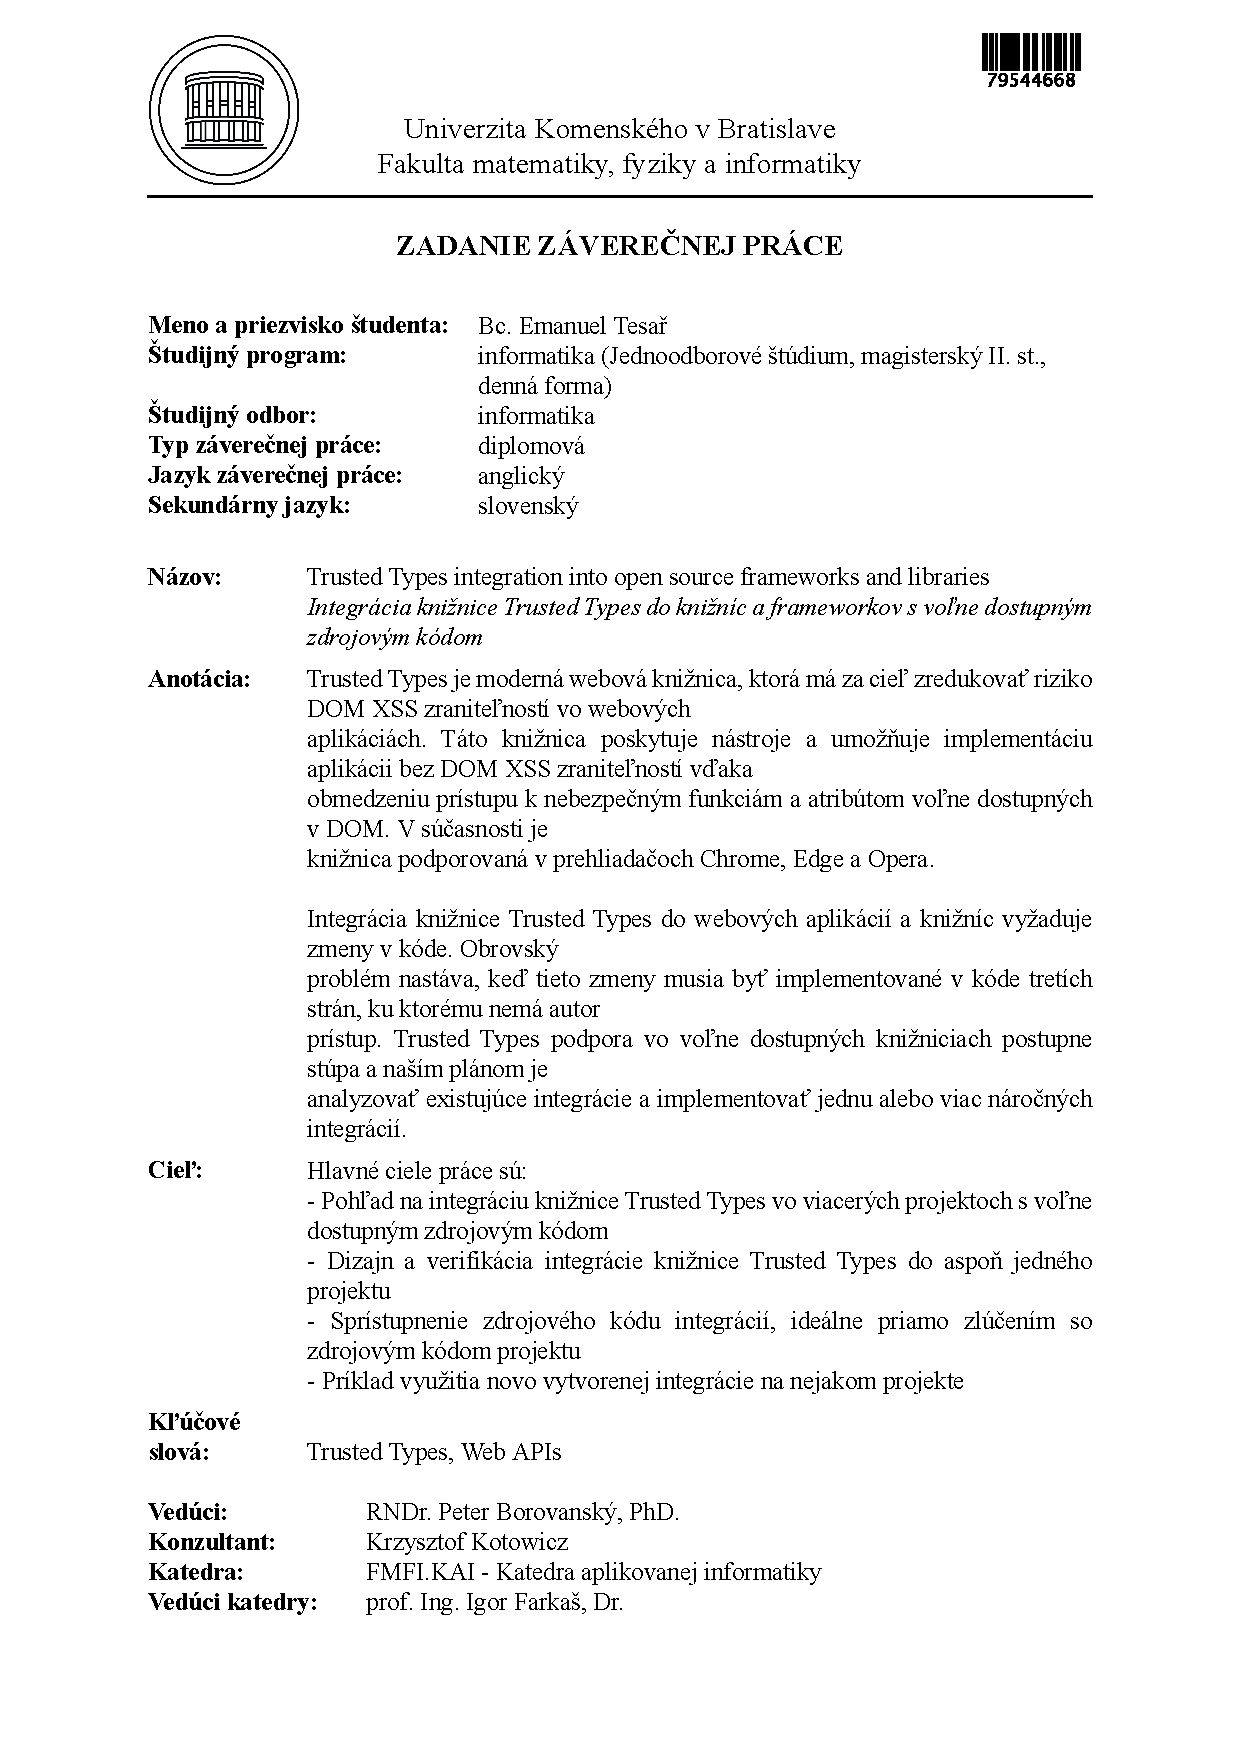
\includegraphics[width=1.1\textwidth]{images/zadanie}

\hspace{-2cm}
\includegraphics[width=1.1\textwidth]{images/zadanie-en}

% --- Koniec zadania

\frontmatter

% -------------------
%   Poďakovanie - nepovinné
% -------------------
\setcounter{page}{3}
\newpage
~

\vfill
{\bf Acknowledgments: I want to thank everyone for motivating me to finish the studies and the
  support when I was struggling. Big thanks to my consultalt Krzysztof Kotowicz for all the support,
  friendliness and help.}

% --- Koniec poďakovania

% -------------------
%   Abstrakt - Slovensky
% -------------------
\newpage
\section*{Abstrakt}

Trusted Types je moderná webová knižnica, ktorá má za cieľ zredukovať riziko DOM XSS zraniteľností
vo webových aplikáciách. Táto knižnica poskytuje nástroje a umožňuje implementáciu aplikácii bez DOM
XSS zraniteľností vďaka obmedzeniu prístupu k nebezpečným funkciám a atribútom voľne dostupných v
DOM. V súčasnosti je knižnica podporovaná v prehliadačoch Chrome, Edge a Opera.

Integrácia knižnice Trusted Types do webových aplikácií a knižníc vyžaduje zmeny v kóde. Obrovský
problém nastáva, keď tieto zmeny musia byť implementované v kóde tretích strán, ku ktorému nemá
autor prístup. Trusted Types podpora vo voľne dostupných knižniciach postupne stúpa a naším plánom
je analyzovať existujúce integrácie a implementovať jednu alebo viac náročných integrácií.

\paragraph*{Kľúčové slová: Trusted Types, Web APIs}
% --- Koniec Abstrakt - Slovensky


% -------------------
% --- Abstrakt - Anglicky
% -------------------
\newpage
\section*{Abstract}

Trusted Types is a modern Web API which aims to reduce DOM XSS attack surface in web applications.
They give you the tools to write and maintain applications free of DOM XSS vulnerabilities by making
the dangerous web API secure by default. Currently, they are supported in Chrome, Edge and Opera.

Integrating Trusted Types in web applications and libraries requires code changes. The major problem
is when these changes need to be made in third party code which you don't have access to and you
can't easily modify. Trusted Types support in open source projects is gradually improving and our
plan is to analyze these integrations and implement one or more of the challenging ones.

\paragraph*{Keywords: Trusted Types, Web APIs}

% --- Koniec Abstrakt - Anglicky

% -------------------
% --- Predhovor - v informatike sa zvacsa nepouziva
% -------------------
%\newpage 
%\thispagestyle{empty}
%
%\huge{Predhovor}
%\normalsize
%\newline
%Predhovor je všeobecná informácia o práci, obsahuje hlavnú charakteristiku práce 
%a okolnosti jej vzniku. Autor zdôvodní výber témy, stručne informuje o cieľoch 
%a význame práce, spomenie domáci a zahraničný kontext, komu je práca určená, 
%použité metódy, stav poznania; autor stručne charakterizuje svoj prístup a svoje 
%hľadisko. 
%
% --- Koniec Predhovor


% -------------------
% --- Obsah
% -------------------

\newpage

\tableofcontents

% ---  Koniec Obsahu

% -------------------
% --- Zoznamy tabuliek, obrázkov - nepovinne
% -------------------

\newpage

% \listoffigures
% \listoftables

% ---  Koniec Zoznamov

\mainmatter

\input definitions.tex

\input intro.tex

\input tt-integration-process.tex

\input preprocessor-integration.tex

\input web-framework-integrations.tex

\input testing-integrations.tex

\input conclusion.tex

% -------------------
% --- Bibliografia
% -------------------


\newpage

\backmatter

\thispagestyle{empty}
\nocite{*}
\clearpage

\bibliographystyle{plain}
\bibliography{literatura}

%Prípadne môžete napísať literatúru priamo tu
%\begin{thebibliography}{5}

%\bibitem{br1} MOLINA H. G. - ULLMAN J. D. - WIDOM J., 2002, Database Systems, Upper Saddle River : Prentice-Hall, 2002, 1119 s., Pearson International edition, 0-13-098043-9

%\bibitem{br2} MOLINA H. G. - ULLMAN J. D. - WIDOM J., 2000 , Databasse System implementation, New Jersey : Prentice-Hall, 2000, 653s., ???

%\bibitem{br3} ULLMAN J. D. - WIDOM J., 1997, A First Course in Database Systems, New Jersey : Prentice-Hall, 1997, 470s., 

%\bibitem{br4} PREFUSE, 2007, The Prefuse visualization toolkit,  [online] Dostupné na internete: <http://prefuse.org/>

%\bibitem{br5} PREFUSE Forum, Sourceforge - Prefuse Forum,  [online] Dostupné na internete: <http://sourceforge.net/projects/prefuse/>

%\end{thebibliography}

%---koniec Referencii

% -------------------
%--- Prilohy---
% -------------------

%Nepovinná časť prílohy obsahuje materiály, ktoré neboli zaradené priamo  do textu. Každá príloha sa začína na novej strane.
%Zoznam príloh je súčasťou obsahu.
%
%\input appendixA.tex

%\input appendixB.tex

\end{document}
